\documentclass[twocolumn]{article}

\usepackage[utf8]{inputenc}
\usepackage{lmodern}
\usepackage[T1]{fontenc}
\usepackage[catalan]{babel}
\usepackage{mathtools}
\usepackage{float}
\usepackage{csvsimple}
\providecommand{\abs}[1]{\lvert#1\rvert}

\usepackage{fancyhdr}

\usepackage{authblk}

\usepackage[backend=biber,style=phys]{biblatex}
\addbibresource{.bib}

% \usepackage{multirow}
% \usepackage[table,xcdraw]{xcolor}

% \usepackage{graphicx}
% \usepackage{caption}
% \usepackage{subcaption}

% \usepackage[a4paper]{geometry}
% \geometry{top=3cm, bottom=3.3cm, left=3cm, right=3cm}


\title{Entanglement Entropy and Holography}
\author{Ferran Rodríguez Mascaró}
\date{}

\begin{document}

\maketitle{}


% \begin{abstract}
    
% \end{abstract}


\section{Introducció}

\subsection{Equació d'Einstein}

L'equació d'Einstein del camp en dimensió $D$ és
\begin{equation}
    R_{ab} - \frac{1}{2} g_{ab} R + \Lambda g_{ab} = 8 \pi G T_{ab} \ ,
\label{eq:Einstein}
\end{equation}
on $R_{ab}$ és el tensor de Richi\footnote{Els índexs llatins es defineixen com $a,b,c...={0,1,...,D-1}$}, $g_{ab}$ la mètrica\footnotemark, $R$ l'escalar de Richi, $\Lambda$ la constant cosmològica, $G$ la constant de Newton i $T_{ab}$ el tensor d'energia-moment. La podem representar utilitzant el tensor d'Einstein, $G_{ab}$:
\footnotetext{Utilitzem la signatura $(-,+,+,...,+)$}
\begin{equation}
    G_{ab} + \Lambda g_{ab} = 8 \pi G T_{ab} \ .
\label{eq:Einstein2}
\end{equation}
Descriu com la forma de l'espaitemps fa que es mogui la matèria i com aquesta deforma l'espaitemps.

Veiem que és una equació de segon ordre respecte el temps i l'espai, al ser relativista, ja que $R_{ab} \sim \{ \partial \Gamma , \Gamma \} \sim \{ \partial^2 g, \partial g, g \}$. A l'esquerra de l'igualtat tenim una equació dinàmica per la mètrica, que ens diu com actua la gravetat segons la distribució de matèria, representada pel tensor $T_{ab}$.

\subsection{Solucions de Buit. Solucions Maximalment Simètriques}

En les solucions de l'equació d'Einstein de buit, el tensor d'energia-moment és nul. El camp gravitatori no s'acbola a res, només a si mateix.
\begin{equation}
    G_{ab} + \Lambda g_{ab} = 0 \ .
\label{eq:SolBuit}
\end{equation}

Les solucions maximalment simètrics son el subconjunt de solucions de buit en les que s'admeten el major nombre de vectors de Killing o isometries possibles ($\frac{D(D+1)}{2}$). Aquestes tenen un tensor de Riemann simètric amb la forma
\begin{equation}
    R_{abcd} = k ( g_{ac} g_{bd} - g_{ad} g_{bc} ) \ , \ k \sim R f(D) \ .
\label{eq:SolMaximRiemann}
\end{equation}

Dins d'aquestes solucions, tindrem espaitemps amb diferents propietats segons el valor de la constant cosmològica:
\begin{itemize}
    \item $\Lambda = 0$: Espaitemps de Minkowski.
    \item $\Lambda > 0$: Espaitemps de de Sitter.
    \item $\Lambda < 0$: Espaitemps d'anti-de Sitter.
\end{itemize}

\subsection{Espaitemps d'Anti-de Sitter}

En l'espaitemps d'anti-de Sitter, la constant cosmològica és negativa, i definim el tensor de Riemann agafant $k=-\frac{1}{L^2}$. Per tant, aquest tindrà una forma tal que
\begin{equation}
    R_{abcd} = -\frac{1}{L^2} ( g_{ac} g_{bd} - g_{ad} g_{bc} ) \ .
\label{AdSRiemann}
\end{equation}

Es troba que per a que aquest tipus d'espaitemps sigui solució de l'equació d'Einstein \ref{eq:Einstein}, la constant cosmològica ha de valer
\begin{equation}
    \Lambda = - \frac{(D-1)(D-2)}{2L^2} \ .
\label{eq:AdSLambda}
\end{equation}

En les coordenades del \textit{patch} de Pointcaré, la mètrica d'anti-de Sitter de dimensió $D$ es defineix com
\begin{equation}
    ds_{AdS_D}^2 = \frac{L^2}{z^2} ( -dt^2 + dz^2 + dx_1^2 + dx_2^2 + ... + dx_{D-2}^2 ) \ ,
\label{eq:MetPointcareAdS}
\end{equation}
amb $z \in (0,+\infty)$ i $t,x \in (-\infty,+\infty)$, que correspon a un espaitemps de Minkowski però amb un factor $\frac{L^2}{z^2}$.

Fixant la coordenada $z$, tenim superfícies d'espaitemps de Minkowski amb un factor de pes $\frac{L^2}{z^2}$, determinat per $z$, representat en la figura \ref{fig:Superficies_z}.
\begin{figure}[h!]
    \centering
    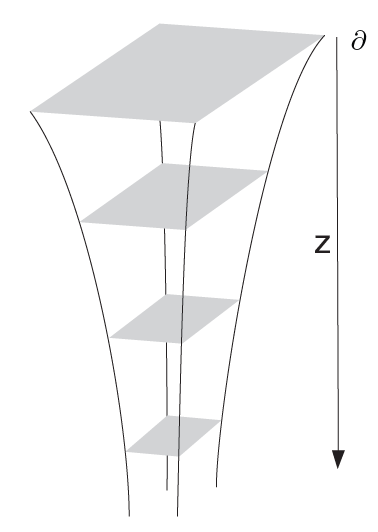
\includegraphics[scale=0.5]{../Imatges/Captura_Superficies_z.png}
\caption{Representació de diferents superfícies d'espaitemps de Minkowski dins de l'espaitemps d'anti-de Sitter segons el valor de la coordenada $z$.}
\label{fig:Superficies_z}
\end{figure}

En coordenades esfèriques, la mètrica es pot expressar com
\begin{equation}
    ds_{AdS_D}^2 = \left [ - \left ( 1 + \frac{r^2}{L^2} \right ) dt^2 + \frac{dr^2}{\left ( 1+ \frac{r^2}{L^2} \right )} + r^2 d \Omega_{D-2}^2 \right ] \ .
\label{eq:MetEsfAdS}
\end{equation}
La coordenada $r$ es relaciona amb $z$ segons $r \sim \frac{1}{z}$. Considerem que $z = \delta \ll 1$, però no nul, que llavors $ds^2 \to \infty$.






% \printbibliography

\end{document}